\chapter{Свойства гармонических функций: теорема о потоке, теоремы о среднем по сфере и по шару, принцип максимума, теорема Лиувилля.}
\label{cha:18}

\section*{Свойства гармонических функций}

\begin{remem}\label{lec:18/remem:1}
	Напомним несколько важных определений:
	\begin{enumerate}
		\item 
			Функция $ u(x) \in C^2(\Omega)$ называется \blue{гармонической}, если $\Delta u = 0$.
		\item
			Фундаментальное решение оператора Лапласса имеет вид:
			$$\varepsilon(x) = 
			\begin{cases}
				\dfrac{1}{2\pi} \log|x|, \; x \in \mathbb{R}^2 \\
				-\dfrac{1}{4\pi |x|}, \; \in \mathbb{R}^3
			\end{cases}  \Delta \varepsilon(x) = \delta(x)$$
	\end{enumerate}
\end{remem}
Введем обозначения:
\begin{itemize}
	\item[$\bullet$] 
		сфера: $\displaystyle S_{x_0}^{R} = \lbrace |x - x_0| = R \rbrace$, 
		$|S_{x_0}^{R}| = 
		\begin{cases}
			2\pi R, \; x \in \mathbb{R}^2 \\
			4\pi R^2, \; x \in \mathbb{R}^3 
		\end{cases}$
	\item[$\bullet$] 
		шар: $\displaystyle B_{x_0}^{R} = \lbrace |x - x_0| \leq R \rbrace$, $|B_{x_0}^{R}| = 
		\begin{cases}
			\pi R^2, \; x \in \mathbb{R}^2 \\
			\frac{4}{3}\pi R^3, \; x \in \mathbb{R}^3 
		\end{cases}$
\end{itemize}

\begin{theorem}[\red{Теорема о потоке для гармонической функции}]
	$\;$\\
	Пусть $ \Delta u = 0$, $ x \in \Omega, $ тогда:
	$ \displaystyle \iint \limits_{\Omega} \Delta u d\bar{x} = \oint\limits_{\partial \Omega} \dfrac{\partial u}{\partial \bar{n}} d\sigma = 0$.
\end{theorem}
\begin{Proof}
	Следует из теоремы о потоке для обычной функции.
\end{Proof}

\begin{theorem}[\red{Теорема о среднем на сфере}]
	$\;$\\
	Пусть $ \Delta u = 0$, $x \in B_{x_0}^R$, тогда 
	$\displaystyle u(x_0) = \dfrac{1}{|S_{x_0}^R|} \oint\limits_{S_{x_0}^R} u(x)d\sigma$
\end{theorem}
\begin{Proof}
	Докажем для $\mathbb{R}^3$, доказательство для $\mathbb{R}^2$ аналогично.

	Применим 2-ую формулу Грина для $ u(x), \; \varepsilon(x - x_0)$:
	$$\begin{gathered}
		\iint \limits_{B_{x_0}^R}( \underbrace{\Delta \varepsilon(x - x_0)}_{= \delta(x - x_0)}u(x) - \underbrace{\Delta u(x)}_{= 0}\varepsilon(x - x_0)dx 
		= \\
		= \iint \limits_{B_{x_0}^R} \underbrace{\delta(x - x_0)u(x)}_{=\delta(x - x_0)u(x_0)}dx
		= u(x_0)\underbrace{\iint \limits_{B_{x_0}^R} \delta(x - x_0)dx}_{=1} = u(x_0) 
		= \\
		= \oint\limits_{S_{x_0}^R}\left(u(x)\dfrac{\partial \varepsilon(x - x_0)}{\partial \bar{n}} - \varepsilon(x - x_0) \dfrac{\partial u(x)}{\partial \bar{n}}\right)d\sigma = \\
		= \oint\limits_{S_{x_0}^R} \left(u(x) \dfrac{\partial}{\partial \rho}(-\dfrac{1}{4\pi \rho}) + \dfrac{1}{4\pi \rho} \dfrac{\partial u(x)}{\partial \bar{n}} \right) \Big|_{\rho = R}d\sigma = \\
		= \dfrac{1}{4\pi R^2} \oint\limits_{S_{x_0}^R} u(x)d\sigma + \dfrac{1}{4\pi R} \oint\limits_{S_{x_0}^R} \underset{= 0}{\dfrac{\partial u(x)}{\partial \bar{n}}}d\sigma = \dfrac{1}{|S_{x_0}^R|} \oint\limits_{S_{x_0}^R} u(x)d\sigma
	\end{gathered}$$
\end{Proof}

\vspace{0.5cm}
\begin{theorem}[\red{Теорема о среднем по шару}]
	$\;$\\
	Пусть $ \Delta u = 0$, $x \in B_{x_0}^R$, тогда 
	$\displaystyle u(x_0) = \dfrac{1}{|B_{x_0}^R|} \iint \limits_{B_{x_0}^R} u(x)d\bar{x}$.
\end{theorem}
\begin{Proof}
	Распишем преобразования:
	$$\iint \limits_{B_{x_0}^R} u(x)d\bar{x} = \int\limits_{0}^R (\oint\limits_{S_{x_0}^R} u(x)d\sigma)d\rho = \int\limits_{0}^R u(x_0) |S_{x_0}^R| d\rho = u(x_0) \int\limits_{0}^R \oint\limits_{S_{x_0}^R} 1 d\sigma d\rho = u(x_0)|B_{x_0}^R|$$
	Тогда $\displaystyle u(x_0) = \dfrac{1}{|B_{x_0}^R|} \iint \limits_{B_{x_0}^R} u(x)d\bar{x}$.
\end{Proof}

\vspace{1cm}
\begin{theorem}[\red{Строгий принцип максимума}]
	Пусть $ \Delta u \equiv 0, \; x \in \Omega, \; u \not\equiv const$ и $M = \underset{\partial \Omega}{max}\;u(x), \; m = \underset{\partial \Omega}{min}\;u(x)$, тогда $\forall \; x \in \Omega \; m < u(x) < M.$
\end{theorem}
\begin{Proof}
	Докажем, что, если $ u(x) $ достигает max во внутренней точке области $ \Omega$, то $u(x) \equiv const$. 

	\begin{multicols}{2}
		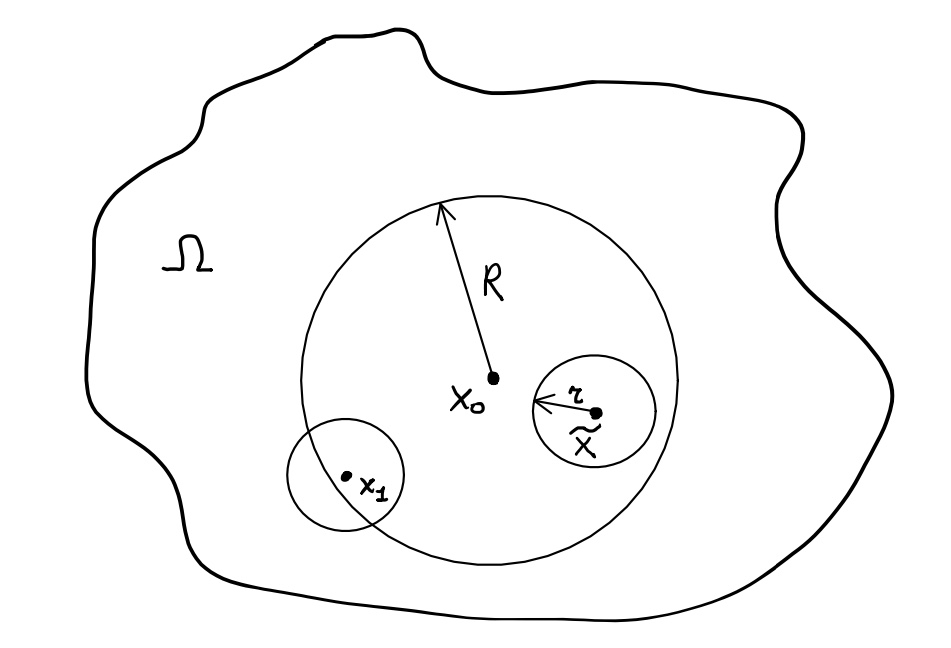
\includegraphics[scale=0.25]{cha18im1}
		\columnbreak

		Положим $ M = \underset{\bar{\Omega}}{max}\;u(x) $. 

		Пусть $ \exists x_0 \hspace{-4pt} \in \hspace{-4pt} \Omega $ - такая внутренняя точка $ \Omega$, что $u(x_0) = M$.

		$x_0 $ - внутренняя, тогда $\exists B_{x_0}^R \subset \Omega$.

		Пусть $u(x) \hspace{-5pt}\not\equiv\hspace{-5pt} M $ в $ B_{x_0}^R$, а также пусть  \\$\;\;\;\;\;\;$ $u(x) \leq M \; \forall \; x \in \Omega$.

		Тогда $\exists \tilde{x} \in B_{x_0}^R: \; u(\tilde{x}) < M$.

		$u(x) $ -- непрерывная, значит \\$\exists B_{\tilde{x}}^r: \; u(x) < M $ в $ B_{\tilde{x}}^r$.
	\end{multicols}
	Применим теорему о среднем по шару $ B_{x_0}^R: $
	$$\begin{gathered}
		u(x_0) = M = \dfrac{1}{B_{x_0}^R} \iint \limits_{B_{x_0}^R}u(x)d\bar{x} = \dfrac{1}{B_{x_0}^R}\left( \iint \limits_{B_{\tilde{x}}^r}\underbrace{u(x)}_{< M}d\bar{x} + \iint \limits_{B_{x_0}^R \setminus B_{\tilde{x}}^r} \underbrace{u(x)}_{\leq M}d\bar{x}\right) < \\
		< \dfrac{M}{|B_{x_0}^R|} ( |B_{\tilde{x}}^r| + |B_{x_0}^R| - |B_{\tilde{x}}^r| ) = M \text{ -- противоречие} \; \Rightarrow \;  u(x) \equiv M \text{ в } B_{x_0}^R.
	\end{gathered}$$
\end{Proof}

\begin{theorem}[\red{$ \infty $ дифференцируемость гармонической функции}]
	$\;$\\
	Пусть $ \Delta u = 0, \; x \in \Omega$, тогда $u(x) \in C^{\infty}(\Omega)$.
\end{theorem}
\begin{Proof}
	Применим 2-ую формулу Грина для $ u(y) $ и $ \varepsilon(y - x)$:
	$$\begin{gathered}
		\iint \limits_{\Omega}(u(y)\underbrace{\Delta_y\varepsilon(y - x)}_{\delta(y - x)} - \varepsilon(y - x)\underset{= 0}{\Delta_y u(y)})dy = \oint\limits_{\partial \Omega} (u(y) \dfrac{\partial \varepsilon(y - x)}{\partial \bar{n_y}} - \varepsilon(y - x) \dfrac{\partial u(y)}{\partial \bar{n_y}})d\sigma_y \\
		u(x) = \oint\limits_{\partial \Omega}\left( u(y) \dfrac{\partial \varepsilon(y - x)}{\partial \bar{n_y}} - \varepsilon(y - x) \dfrac{\partial u(y)}{\partial \bar{n_y}}\right)d\sigma_y\\
		\dfrac{\partial u(x)}{\partial x_i} =  \oint\limits_{\partial \Omega}\left( u(y) \dfrac{\partial}{\partial x_i}(\dfrac{\partial \varepsilon(y - x)}{\partial \bar{n_y}}) - \dfrac{\partial \varepsilon(y - x)}{\partial x_i} \dfrac{\partial u(y)}{\partial \bar{n_y}}\right)d\sigma_y \\
		\dfrac{\partial^{|\alpha|} u(x)}{\partial x^{\alpha}} = - || -, \text{ т.к. } \varepsilon(y - x) \in C^{\infty} \text{ при } x \neq y.
	\end{gathered}$$
\end{Proof}

\begin{theorem}[\red{Теорема Луивилля}]
	$\;$\\
	Пусть $ \Delta u = 0 \text{ в } \mathbb{R}^n$ и $u(x) \geq c \text{ в } \mathbb{R}^n$, тогда $u \equiv const$.
\end{theorem}
\begin{Proof}
	Введем вспомогательную функцию $ \upsilon(x) = u(x) - c \geq 0$, тогда $\Delta \nu(x) = 0$ и $\Delta(\dfrac{\partial \nu(x)}{\partial x_i})$. Применим теорему о среднем по шару $ B_{x_0}^R $:
	$$\dfrac{\partial \nu(x_0)}{\partial x_i} = \dfrac{1}{|B_{x_0}^R|} \iint\limits_{B_{x_0}^R} \dfrac{\partial \nu(x)}{\partial x_i} d\bar{x}$$
	По формуле Гаусса - Остроградского:
	$$\dfrac{1}{|B_{x_0}^R|} \oint\limits_{S_{x_0}^R} \underbrace{\nu(x)}_{\geq 0}n_id\sigma = \dfrac{n_i(x^*)}{|B_{x_0}^R|} \oint\limits_{S_{x_0}^R} \nu(x)d\sigma = \dfrac{n_i(x^*)}{|B_{x_0}^R|}\nu(x_0)  |S_{x_0}^R|$$
	Тогда $\displaystyle |\dfrac{\partial \nu(x_0)}{\partial x_i}| \leq \dfrac{c}{R} \underset{R \longrightarrow \infty}{\longrightarrow} 0$. Значит:
	$$\dfrac{\partial \nu(x_0)}{\partial x_i} = 0 \; \Rightarrow \;  \dfrac{\partial \nu(x)}{\partial x_i} = 0, \; i = 1, \ldots, n \; \Rightarrow \;  v \equiv const \; \Rightarrow \;  u \equiv const$$
\end{Proof}









